% NplusPrep project handover.
% Build (XeLaTeX, TeX Live): latexmk -xelatex handover.tex
% Fonts and packages: tlmgr install lexend sourceserif sourcesans sourcecodepro underscore fontawesome5 tcolorbox
%   pdfcol tikzfill environ trimspaces enumitem titlesec fancyhdr caption
% Screenshots in img/ are rendered from the app's own screens and painters
% (see section "Updating the screenshots").
\documentclass[11pt,a4paper]{article}

% ---------------------------------------------------------------- fonts
\usepackage{fontspec}
\setmainfont{SourceSerif4}[
  Extension=.otf, UprightFont=*-Regular, BoldFont=*-Semibold,
  ItalicFont=*-RegularIt, BoldItalicFont=*-SemiboldIt, Numbers=Lining]
\setsansfont{SourceSans3}[
  Extension=.otf, UprightFont=*-Regular, BoldFont=*-Semibold,
  ItalicFont=*-RegularIt, BoldItalicFont=*-SemiboldIt]
\newfontfamily\lexend{LexendDeca}[Extension=.ttf, UprightFont=*-Regular]
\setmonofont{SourceCodePro}[
  Extension=.otf, UprightFont=*-Regular, BoldFont=*-Semibold, ItalicFont=*-RegularIt, Scale=0.86]
\usepackage{fontawesome5}

% ---------------------------------------------------------------- layout
\usepackage[a4paper,top=24mm,bottom=24mm,left=22mm,right=22mm,headheight=14pt]{geometry}
\usepackage[table]{xcolor}
\definecolor{brand}{HTML}{195DE6}
\definecolor{ink}{HTML}{1E293B}
\definecolor{subtle}{HTML}{64748B}
\definecolor{rule}{HTML}{CBD5E1}
\definecolor{wash}{HTML}{F1F5FB}
\definecolor{okgreen}{HTML}{16A34A}
\definecolor{amber}{HTML}{D97706}
\definecolor{alert}{HTML}{DC2626}
\color{ink}
\usepackage{microtype}
\usepackage{parskip}
\setlength{\parskip}{0.55em}
\usepackage{graphicx}
\graphicspath{{img/}}
\usepackage{booktabs,tabularx,array,longtable,xltabular}
\setlength{\LTpre}{0.4em}\setlength{\LTpost}{0.2em}
\usepackage{enumitem}
\setlist{itemsep=0.15em,topsep=0.3em}
\usepackage{caption}
\captionsetup{font={small,sf},labelfont={bf,color=brand},textfont={color=subtle},skip=6pt}
\usepackage{float}
\usepackage{tikz}
\usetikzlibrary{arrows.meta,positioning,calc,shapes.geometric}
\usepackage[most]{tcolorbox}
\usepackage{listings}
\usepackage{titlesec}
\usepackage{fancyhdr}
\PassOptionsToPackage{hyphens}{url}\usepackage[hidelinks]{hyperref}
\hypersetup{colorlinks=true,linkcolor=brand,urlcolor=brand,
  pdftitle={NplusPrep: Project Handover},pdfauthor={NplusPrep}}

% ---------------------------------------------------------------- headings
\titleformat{\section}{\sffamily\bfseries\LARGE\color{ink}}
  {\colorbox{brand}{\makebox[1.6em]{\color{white}\thesection}}}{0.6em}{}
  [\vspace{-0.4em}\color{rule}\rule{\linewidth}{0.6pt}]
\titleformat{\subsection}{\sffamily\bfseries\Large\color{ink}}{\color{brand}\thesubsection}{0.7em}{}
\titleformat{\subsubsection}{\sffamily\bfseries\large\color{ink}}{}{0em}{}
\titlespacing*{\section}{0pt}{1.6em}{1em}
\titlespacing*{\subsection}{0pt}{1.4em}{0.5em}
\newcommand{\sectionbreak}{\clearpage}

\pagestyle{fancy}
\fancyhf{}
\renewcommand{\headrulewidth}{0pt}
\fancyhead[L]{\sffamily\footnotesize\color{subtle}NplusPrep \textbullet\ Project handover}
\fancyhead[R]{\sffamily\footnotesize\color{subtle}\nouppercase{\leftmark}}
\fancyfoot[C]{\sffamily\footnotesize\color{subtle}\thepage}
\renewcommand{\sectionmark}[1]{\markboth{#1}{}}

% ---------------------------------------------------------------- tables
\renewcommand{\arraystretch}{1.3}
\newcolumntype{L}{>{\raggedright\arraybackslash}X}
\newcolumntype{P}[1]{>{\raggedright\arraybackslash}p{#1}}
\newcommand{\thead}[1]{\sffamily\bfseries\small\color{brand}#1}
% A table: \begin{tbl}{colspec} header row \\ \midrule rows \end{tbl}
\newenvironment{tbl}[1]
  {\par\small\rowcolors{2}{wash}{white}\xltabular{\linewidth}{@{}#1@{}}\toprule\rowcolor{white}}
  {\bottomrule\endxltabular\par}

% ---------------------------------------------------------------- inline code
\usepackage[strings]{underscore}
% Long paths and commands may break after / . - = (only inside \code).
\newXeTeXintercharclass\codebreak
\XeTeXcharclass`\/=\codebreak \XeTeXcharclass`\.=\codebreak
\XeTeXcharclass`\-=\codebreak \XeTeXcharclass`\==\codebreak
\XeTeXinterchartoks\codebreak 0 = {\penalty50\relax}
\newcommand{\codebs}{\symbol{92}\penalty50\relax}
\newcommand{\code}[1]{\texttt{\let\textbackslash\codebs\XeTeXinterchartokenstate=1 #1\XeTeXinterchartokenstate=0 }}
\setlength{\emergencystretch}{2em}
\newcommand{\key}[1]{\tikz[baseline=(k.base)]\node[draw=rule,fill=wash,rounded corners=2pt,inner sep=2pt,font=\sffamily\footnotesize](k){#1};}

% ---------------------------------------------------------------- code blocks
\lstdefinestyle{shell}{
  basicstyle=\ttfamily\small\color{ink}, columns=fullflexible, keepspaces=true,
  backgroundcolor=\color{wash}, frame=leftline, framerule=2.5pt, rulecolor=\color{brand},
  xleftmargin=8pt, framexleftmargin=8pt, aboveskip=0.8em, belowskip=0.8em,
  commentstyle=\color{subtle}\itshape, comment=[l]{\#}, morecomment=[l]{//},
  breaklines=true, postbreak=\mbox{\textcolor{subtle}{$\hookrightarrow$}\space},
  showstringspaces=false, upquote=true}
\lstnewenvironment{shell}{\lstset{style=shell}}{}

% ---------------------------------------------------------------- callouts
\newtcolorbox{callout}[3]{enhanced, breakable, colback=#1!6, colframe=#1,
  boxrule=0pt, leftrule=3pt, arc=2pt, left=10pt, right=10pt, top=6pt, bottom=6pt,
  fontupper=\small, before upper={{\sffamily\bfseries\color{#1}#2\enspace#3.}\enspace}}
\newenvironment{note}{\begin{callout}{brand}{\faInfoCircle}{Note}}{\end{callout}}
\newenvironment{tip}{\begin{callout}{okgreen}{\faLightbulb[regular]}{Tip}}{\end{callout}}
\newenvironment{important}{\begin{callout}{amber}{\faExclamationCircle}{Important}}{\end{callout}}
\newenvironment{warning}{\begin{callout}{alert}{\faExclamationTriangle}{Warning}}{\end{callout}}

% ---------------------------------------------------------------- figures
% A phone screenshot with a thin frame.
\newcommand{\phone}[2][0.3]{\tikz[baseline]\node[draw=rule,line width=0.6pt,inner sep=0pt]{\includegraphics[width=#1\textwidth]{#2}};}
% Four moments of one explanation (start, two in-between, end), left to right.
% The Replay button column is trimmed off the panel captures.
\newcommand{\frameimg}[2]{\raisebox{-0.5\height}{\includegraphics[width=0.228\linewidth,trim=0 0 105 0,clip]{explain_#1_#2}}}
\newcommand{\framearrow}{\hfill{\color{brand}\small\faAngleRight}\hfill}
\newcommand{\filmstrip}[2]{%
  \par\noindent\begin{minipage}{\linewidth}
  {\sffamily\bfseries\small #2}\par\vspace{3pt}\noindent
  \frameimg{#1}{0}\framearrow\frameimg{#1}{1}\framearrow\frameimg{#1}{2}\framearrow\frameimg{#1}{4}%
  \end{minipage}\par\medskip}
% TikZ styles shared by the diagrams.
\tikzset{
  box/.style={draw=brand, fill=wash, rounded corners=4pt, font=\sffamily\small,
    align=center, inner sep=6pt, minimum height=2.2em},
  plain/.style={draw=rule, fill=white, rounded corners=4pt, font=\sffamily\small,
    align=center, inner sep=6pt, minimum height=2.2em},
  hot/.style={draw=brand, fill=brand, text=white, rounded corners=4pt, font=\sffamily\small\bfseries,
    align=center, inner sep=6pt, minimum height=2.2em},
  flow/.style={-{Stealth[length=6pt]}, draw=subtle, line width=0.8pt},
  lab/.style={font=\sffamily\scriptsize, text=subtle}}

\begin{document}

% ================================================================ cover
\begin{titlepage}
\newgeometry{top=0mm,bottom=0mm,left=0mm,right=0mm}
\begin{tikzpicture}[remember picture,overlay]
  \fill[brand] (current page.north west) rectangle ([yshift=-108mm]current page.north east);
  \node[anchor=north west, text=white, font=\lexend\fontsize{44}{48}\selectfont]
    at ([xshift=22mm,yshift=-34mm]current page.north west) {NplusPrep};
  \node[anchor=north west, text=white, font=\lexend\fontsize{20}{24}\selectfont]
    at ([xshift=22mm,yshift=-52mm]current page.north west) {Project handover};
  \node[anchor=north west, text=white!80!brand, font=\sffamily\small, text width=95mm]
    at ([xshift=22mm,yshift=-68mm]current page.north west)
    {An offline Android app that trains children for the Mental Ability Test of the JNVST.
     Everything the next owner needs: setup, architecture, how we work, what went wrong and what is still open.};
  \node[anchor=north east] at ([xshift=-22mm,yshift=-22mm]current page.north east)
    {\tcbox[enhanced,colback=white,colframe=white,boxrule=0pt,arc=8pt,left=0pt,right=0pt,top=0pt,bottom=0pt,
      drop fuzzy shadow]{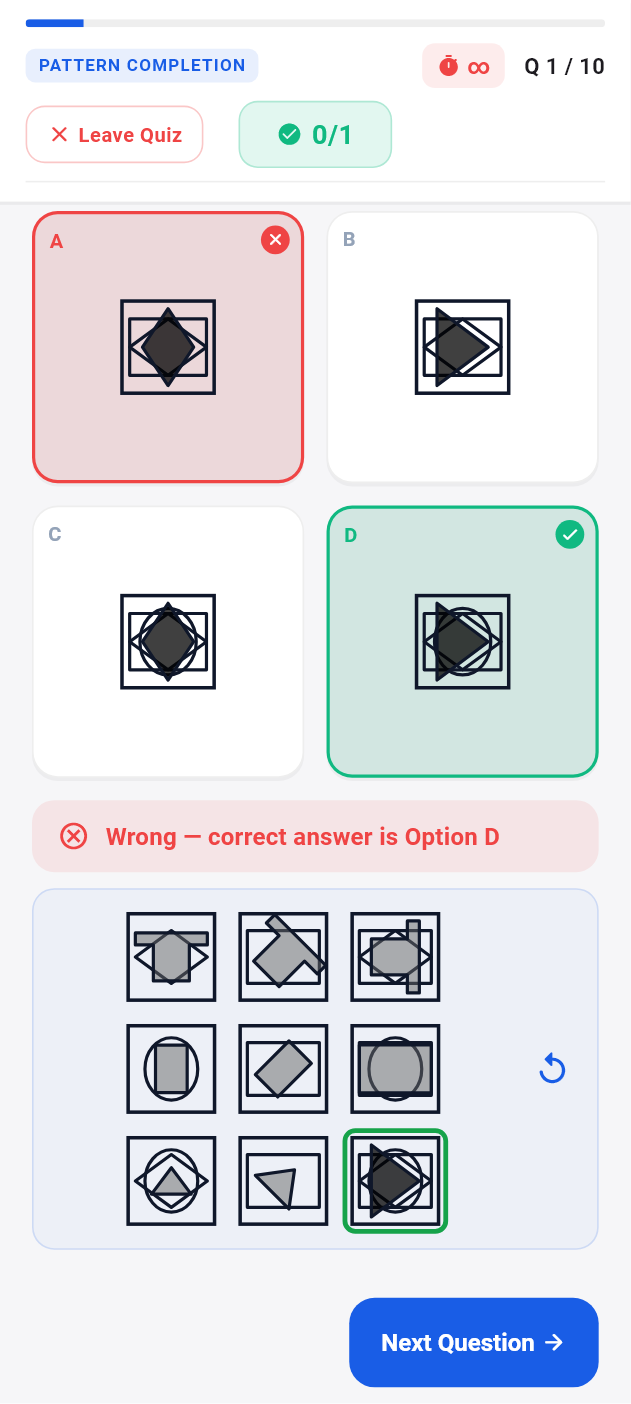
\includegraphics[width=66mm]{screen_quiz_pattern_explained}}};
  \node[anchor=north west, font=\sffamily\normalsize, text=ink, align=left]
    at ([xshift=22mm,yshift=-175mm]current page.north west) {%
    \begin{tabular}{@{}r@{\hspace{1em}}l@{}}
      {\color{subtle}For}   & the incoming project owner \\
      {\color{subtle}From}  & Hari (developer) \\
      {\color{subtle}Date}  & 5 November 2026 \\
      {\color{subtle}State} & beta 9 (\code{v1.0.0-beta.9}), released 4 Nov 2026 \\
      {\color{subtle}Tests} & 365 automated tests, all passing
    \end{tabular}};
  \node[anchor=south west, text width=166mm, font=\sffamily\small, text=subtle] at ([xshift=22mm,yshift=24mm]current page.south west)
    {\textbf{\color{ink}New in beta 9: answer explanations.} After a wrong answer, the rule is acted out on the question's own figures.\par\vspace{4pt}
     \frameimg{series}{0}\framearrow\frameimg{series}{1}\framearrow\frameimg{series}{2}\framearrow\frameimg{series}{4}};
\end{tikzpicture}
\end{titlepage}
\restoregeometry

\setcounter{page}{2}
{\sffamily\small\setlength{\parskip}{0.2em}
\makeatletter\renewcommand{\@dotsep}{1000}\makeatother
\renewcommand{\sectionbreak}{}\tableofcontents}

\vfill
\begin{note}
This document explains the whole project from the ground up: what it is, how to set up a computer to work on it, how it is built, how we work, every major problem we hit and how it was fixed, and how to deal with problems in future. No earlier knowledge of Flutter or Android is assumed.
\end{note}

% ================================================================ 1
\section{The project in one page}

\textbf{What it is.} NplusPrep is an Android app that trains children for the Mental Ability Test of the JNVST, the entrance exam for Jawahar Navodaya Vidyalaya (class 6). The test is 40 picture-based reasoning questions in 10 parts. The app makes unlimited practice questions of the same kinds, checks answers, explains wrong answers with a short animation, adapts to each child's weak topics, and can print exam-style papers for a whole class.

\begin{figure}[H]
\centering
\phone[0.27]{screen_config}\hfill
\phone[0.27]{screen_quiz_pattern}\hfill
\phone[0.27]{screen_quiz_pattern_explained}
\caption{The app in beta 9. Left: the home (config) screen. Middle: a Hard Pattern question. Right: after a wrong answer, the explanation builds the missing cell and frames the correct option in green.}
\end{figure}

\textbf{Who uses it.}

\begin{tbl}{P{0.36\linewidth}L}
\thead{Who} & \thead{What they do} \\ \midrule
Children (about 11 years old; Easy level is for grades 2--3) & Take quiz sessions on a phone or tablet \\
Coordinators / teachers & Set up sessions on the config screen, read results, print papers \\
Mentors & Test builds, report problems in the Notion tracker, review printed papers \\
\end{tbl}

\textbf{Key facts.}
\begin{itemize}
\item \textbf{Fully offline.} No server, no login, no internet. Every question is generated on the device by code; there are no question images or question banks.
\item \textbf{11 topics:} Odd Man Out, Figure Match, Pattern Completion, Figure Series, Analogy, Geo Completion, Mirror Shape, Mirror Text/Clock, Punch Hole, Space Visualisation, Embedded Figure. These match the JNVST parts (Mirror is split into shapes and text).
\item \textbf{3 levels:} Easy (grades 2--3, one change per question), Medium (midway), Hard (real exam level).
\item \textbf{3 languages:} English, Marathi, Hindi.
\item \textbf{Intelligent Bias:} a wrong answer makes that topic come up more often (+2 weight, up to 10); a right answer makes it less frequent ($-1$, down to 1).
\item \textbf{Answer explanations:} after a wrong, skipped or timed-out answer, a short wordless animation acts out the rule on the question's own figures and ends on the correct option framed in green (all 11 topics; section~\ref{sec:explanations}).
\item \textbf{Printed papers:} a coordinator picks a number of students and a language; the app makes a PDF with a differently shuffled 40-question paper per student (one A4 sheet, both sides) and a teacher's answer key.
\end{itemize}

\textbf{Where things are.}

\begin{tbl}{P{0.33\linewidth}L}
\thead{Thing} & \thead{Location} \\ \midrule
Code & \url{https://github.com/harikn2003/mental-ability-app} \\
Releases (APK to install) & \url{https://github.com/harikn2003/mental-ability-app/releases} \\
Bug / feature tracker & Notion: ``Navodaya Mental Ability Issues DB'' (shared Notion workspace) \\
Package name (release app) & \code{com.nplusone.maa.mental_ability_app} \\
Package name (debug app) & \code{com.nplusone.maa.mental_ability_app.debug} (installs beside the release app) \\
\end{tbl}

% ================================================================ 2
\section{Setting up a computer from zero}

The project can be developed on \textbf{Windows 10/11} or \textbf{Linux} (Ubuntu/Debian or Fedora). The setup is deliberately light: \textbf{Visual Studio Code} as the editor and Android's \textbf{command-line tools} instead of Android Studio. That is about 1.5\,GB of downloads and far less memory while working, compared with 3--4\,GB and a heavy IDE. Allow 30--60 minutes, mostly downloads.

\begin{note}
``Visual Studio Code'' (VS Code) is the free, lightweight editor -- not ``Visual Studio'', the large Windows IDE, which is not needed at all.
\end{note}

\subsection{What gets installed}

\begin{tbl}{P{0.3\linewidth}LP{0.25\linewidth}}
\thead{Tool} & \thead{Why} & \thead{From (Windows / Linux)} \\ \midrule
\textbf{Git} & Version control; on Windows also gives \textbf{Git Bash}, used by the release hook & winget / apt or dnf \\
\textbf{VS Code} + \textbf{Flutter extension} & Editor with code completion, run and debug buttons & winget / snap or Microsoft package \\
\textbf{Java 17} (or any 17+) & Android builds run on Java & winget (Temurin) / apt or dnf \\
\textbf{Flutter SDK} (stable) & The app framework; includes Dart & Git clone of the stable branch \\
\textbf{Android SDK command-line tools}: platform-tools (\code{adb}), Android 36, build-tools 36, NDK 27 & Builds and installs the Android app & Google's download, then \code{sdkmanager} \\
\textbf{zenity} (Linux only) & Dialog boxes for the release hook & apt or dnf \\
\end{tbl}

Install locations: Flutter in \code{C:\textbackslash{}src\textbackslash{}flutter} (Windows) or \code{\textasciitilde{}/development/flutter} (Linux); the Android SDK in \code{\%LOCALAPPDATA\%\textbackslash{}Android\textbackslash{}Sdk} (Windows) or \code{\textasciitilde{}/Android/Sdk} (Linux).

Both setup scripts install only what is missing, set the paths, accept the Android licences, install the VS Code extension, can clone the project, switch on the release hook, and finish with \code{flutter doctor}. Both have a dry-run mode that shows what they would do without changing anything.

\subsection{Windows: one-step setup}

Open \textbf{PowerShell} and run:
\begin{shell}
# 1. Get the script (or copy tools\setup_windows.ps1 from the repository)
Invoke-WebRequest https://raw.githubusercontent.com/harikn2003/mental-ability-app/master/tools/setup_windows.ps1 -OutFile setup_windows.ps1

# 2. Run it; it also clones the project into the folder you give
powershell -ExecutionPolicy Bypass -File setup_windows.ps1 -ProjectDir "$HOME\StudioProjects\mental_ability_app"
\end{shell}
\begin{itemize}
\item Windows may ask for permission while installing Git, VS Code and Java: click \textbf{Yes}.
\item Add \code{-DryRun} to see what it would do without changing anything.
\item When it finishes, \textbf{close PowerShell and open a new one} so the new paths take effect, then run \code{flutter doctor}.
\end{itemize}

\subsection{Linux: one-step setup}

Open a terminal and run:
\begin{shell}
# 1. Get the script (or copy tools/setup_linux.sh from the repository)
curl -fsSLO https://raw.githubusercontent.com/harikn2003/mental-ability-app/master/tools/setup_linux.sh

# 2. Run it; it also clones the project into the folder you give
bash setup_linux.sh --project-dir ~/projects/mental_ability_app
\end{shell}
\begin{itemize}
\item It asks for your password (\code{sudo}) to install system packages.
\item Add \code{--dry-run} to see what it would do without changing anything.
\item When it finishes, open a \textbf{new terminal} (or run \code{source \textasciitilde{}/.bashrc}), then run \code{flutter doctor}.
\item To use a phone over USB, add yourself to the \code{plugdev} group once and log out and in: \code{sudo usermod -aG plugdev "\$USER"}.
\end{itemize}

\begin{tip}
On either system, \code{flutter doctor} should show green ticks for Flutter, the Android toolchain and VS Code. Warnings for ``Visual Studio'', ``Chrome'' or ``Linux toolchain'' can be ignored: those are only for desktop and web builds, which this project doesn't use. The first app build downloads a few more Android parts automatically; that is normal.
\end{tip}

\subsection{Open the project in VS Code}

\begin{shell}
code ~/projects/mental_ability_app                 # Linux
code "$HOME\StudioProjects\mental_ability_app"     # Windows (PowerShell)
\end{shell}
\begin{enumerate}
\item VS Code offers to install the \textbf{recommended extensions} (Flutter and Dart, listed in \code{.vscode/extensions.json}): click \textbf{Install}.
\item Pick the device in the bottom-right status bar (your phone, once connected -- see \ref{sec:phone}).
\item Open \code{lib/main.dart} and press \key{F5} to run with debugging, or \key{Ctrl}+\key{F5} to run without. Save a file to hot-reload.
\item \key{Ctrl}+\key{Shift}+\key{P} $\rightarrow$ ``Flutter: Run Flutter Doctor'' checks the setup from inside VS Code.
\end{enumerate}

\begin{important}
The setup scripts switch on the project's \textbf{pre-push release hook} (\code{git config core.hooksPath tools/git-hooks}). If you clone the project another way, run that command once in the new folder (on Linux also \code{chmod +x tools/git-hooks/pre-push}). Without it, pushing master won't offer to make a beta, and the two version files can drift apart.
\end{important}

\subsection{Manual setup (if a script can't be used)}

\subsubsection*{Windows}
\begin{enumerate}
\item Install the tools:
\begin{shell}
winget install --id Git.Git -e
winget install --id Microsoft.VisualStudioCode -e
winget install --id EclipseAdoptium.Temurin.17.JDK -e
\end{shell}
\item Flutter: \code{git clone https://github.com/flutter/flutter.git -b stable C:\textbackslash{}src\textbackslash{}flutter}, then add \code{C:\textbackslash{}src\textbackslash{}flutter\textbackslash{}bin} to your user \code{Path} (Start $\rightarrow$ ``Edit environment variables for your account''). Use a folder \textbf{without spaces}.
\item Android command-line tools: from \url{https://developer.android.com/studio#command-line-tools-only} download ``Command line tools only'' for Windows and unzip so that \code{\%LOCALAPPDATA\%\textbackslash{}Android\textbackslash{}Sdk\textbackslash{}cmdline-tools\textbackslash{}latest\textbackslash{}bin\textbackslash{}sdkmanager.bat} exists. Set the user variable \code{ANDROID_HOME} to \code{\%LOCALAPPDATA\%\textbackslash{}Android\textbackslash{}Sdk}, and add its \code{platform-tools} and \code{cmdline-tools\textbackslash{}latest\textbackslash{}bin} folders to \code{Path}.
\end{enumerate}

\subsubsection*{Linux (Ubuntu/Debian; use \texttt{dnf} and the Fedora package names on Fedora)}
\begin{enumerate}
\item Install the tools:
\begin{shell}
sudo apt-get update
sudo apt-get install -y git curl unzip xz-utils zip libglu1-mesa openjdk-17-jdk zenity
sudo snap install code --classic
\end{shell}
\item Flutter: \code{git clone https://github.com/flutter/flutter.git -b stable \textasciitilde{}/development/flutter}.
\item Android command-line tools: download ``Command line tools only'' for Linux from the same page and unzip so that \code{\textasciitilde{}/Android/Sdk/cmdline-tools/latest/bin/sdkmanager} exists.
\item Add to \code{\textasciitilde{}/.bashrc}, then open a new terminal:
\begin{shell}
export ANDROID_HOME="$HOME/Android/Sdk"
export PATH="$HOME/development/flutter/bin:$ANDROID_HOME/platform-tools:$ANDROID_HOME/cmdline-tools/latest/bin:$PATH"
\end{shell}
\end{enumerate}

\subsubsection*{Both systems, in a new terminal}
\begin{enumerate}
\item Android packages and licences:
\begin{shell}
sdkmanager --licenses
sdkmanager "platform-tools" "platforms;android-36" "build-tools;36.0.0" "ndk;27.0.12077973"
flutter doctor --android-licenses
code --install-extension Dart-Code.flutter
\end{shell}
\item Get the code (on Windows use \code{\$HOME\textbackslash{}StudioProjects\textbackslash{}mental_ability_app} as the folder):
\begin{shell}
git clone https://github.com/harikn2003/mental-ability-app.git ~/projects/mental_ability_app
cd ~/projects/mental_ability_app
flutter pub get
git config core.hooksPath tools/git-hooks
\end{shell}
\end{enumerate}

The project was last built with \textbf{Flutter 3.41.9 (stable)}. Optional: the \textbf{GitHub CLI} (\code{winget install --id GitHub.cli -e} on Windows, \code{sudo apt-get install gh} on Linux, then \code{gh auth login}) checks releases and CI from the terminal.

\subsection{Connect a phone}\label{sec:phone}

The app is tested on a real Android phone (a Nothing Phone (2a), model A142).
\begin{enumerate}
\item On the phone: \textbf{Settings $\rightarrow$ About phone $\rightarrow$ tap ``Build number'' 7 times} to unlock Developer options.
\item \textbf{Settings $\rightarrow$ System $\rightarrow$ Developer options $\rightarrow$ turn on ``USB debugging''} (and ``Wireless debugging'' to work without a cable).
\item \textbf{With a cable:} plug in and accept the ``Allow USB debugging?'' prompt on the phone. On Linux, if \code{adb devices} shows ``no permissions'', check you are in the \code{plugdev} group and reconnect.
\item \textbf{Without a cable (Wi-Fi):} phone and PC on the same Wi-Fi. In Developer options $\rightarrow$ Wireless debugging $\rightarrow$ ``Pair device with pairing code''. On the PC:
\begin{shell}
adb pair <ip>:<pairing-port>     # type the 6-digit code shown on the phone
adb devices                      # the phone should be listed as "device"
\end{shell}
\item Check: \code{adb devices} lists the phone, and \code{flutter devices} shows it.
\end{enumerate}
Wireless debugging switches itself off when the phone sleeps or changes network; if \code{adb devices} is empty, turn it back on (section~\ref{sec:nophone}).

% ================================================================ 3
\section{Daily tasks: run, test, build}

All commands run in the project folder and are the same on Windows and Linux; only paths differ (\code{build\textbackslash{}app\textbackslash{}...} on Windows, \code{build/app/...} on Linux).

\begin{tbl}{P{0.27\linewidth}P{0.36\linewidth}L}
\thead{Task} & \thead{Command} & \thead{Notes} \\ \midrule
Run on the phone (debug, hot reload) & \code{flutter run} & Press \key{r} to reload, \key{R} to restart, \key{q} to quit \\
Install a debug build without running from the PC & \code{flutter build apk --debug}, then \code{adb install -r build\textbackslash{}app\textbackslash{}outputs\textbackslash{}flutter-apk\textbackslash{}app-debug.apk} & Installs as the \textbf{debug} app, beside the release app \\
Open the installed debug app & \code{adb shell monkey -p com.nplusone.maa.mental_ability_app.debug -c android.intent.category.LAUNCHER 1} & \\
Check code style and errors & \code{flutter analyze} & Must say ``No issues found!'' \\
Run all tests & \code{flutter test} & 1--3 minutes; must end ``All tests passed!'' (365 at handover) \\
Run one test file & \code{flutter test test/series_test.dart} & \\
Release build (local check only) & \code{flutter build apk --release} & Output in \code{build\textbackslash{}app\textbackslash{}outputs\textbackslash{}flutter-apk\textbackslash{}app-release.apk} \\
Preview on a phone without installing & \code{dart run tool/phone_preview.dart} & Opens the app in the phone's browser via a QR code; see \code{docs/phone_preview.md} \\
\end{tbl}

If \code{adb} lists the phone twice (once by IP, once by name), add \code{-s <name>} to every \code{adb} command, e.g.\ \code{adb -s adb-000553435000367-g9vzXa._adb-tls-connect._tcp install -r ...}.

% ================================================================ 4
\section{How the app is built}

\subsection{Technology}

\begin{tbl}{P{0.22\linewidth}P{0.3\linewidth}L}
\thead{Layer} & \thead{Technology} & \thead{Why it was chosen} \\ \midrule
Language / framework & \textbf{Dart 3.8 + Flutter} & One codebase; fast 2D canvas drawing, which matters because every figure is drawn by code \\
Drawing & Flutter \textbf{\code{CustomPainter}} classes & All question figures are generated and drawn programmatically: no image assets, works offline \\
Session history & \textbf{Hive} (local database) & Stores the last 30 finished sessions on the device \\
Settings and bias weights & \textbf{shared\_preferences} & Small key-value store: last setup (\code{last_setup_*}), topic weights (\code{bias_weights_*}) \\
Charts & \textbf{fl\_chart} & Score and time charts on result screens \\
Fonts & The theme names Lexend, but no font file ships, so phones show Roboto (Android's default); letter questions name Roboto & Readability for children \\
PDF papers & \textbf{pdf} + \textbf{printing} packages & Builds the A4 PDF and opens Android's print/share dialog \\
State management & Plain \code{setState} & The app is small enough not to need a state library \\
Android build & Gradle 8.14.3, Android Gradle Plugin 8.13.0, Kotlin 2.2.20, Java 17 & Pinned versions that work together (see \ref{sec:buildproblems}) \\
CI / releases & \textbf{GitHub Actions} (\code{.github/workflows/beta-release.yml}) & Builds and publishes the APK when a beta tag is pushed \\
\end{tbl}

\subsection{Screens and how a child moves through them}

\begin{figure}[H]
\centering
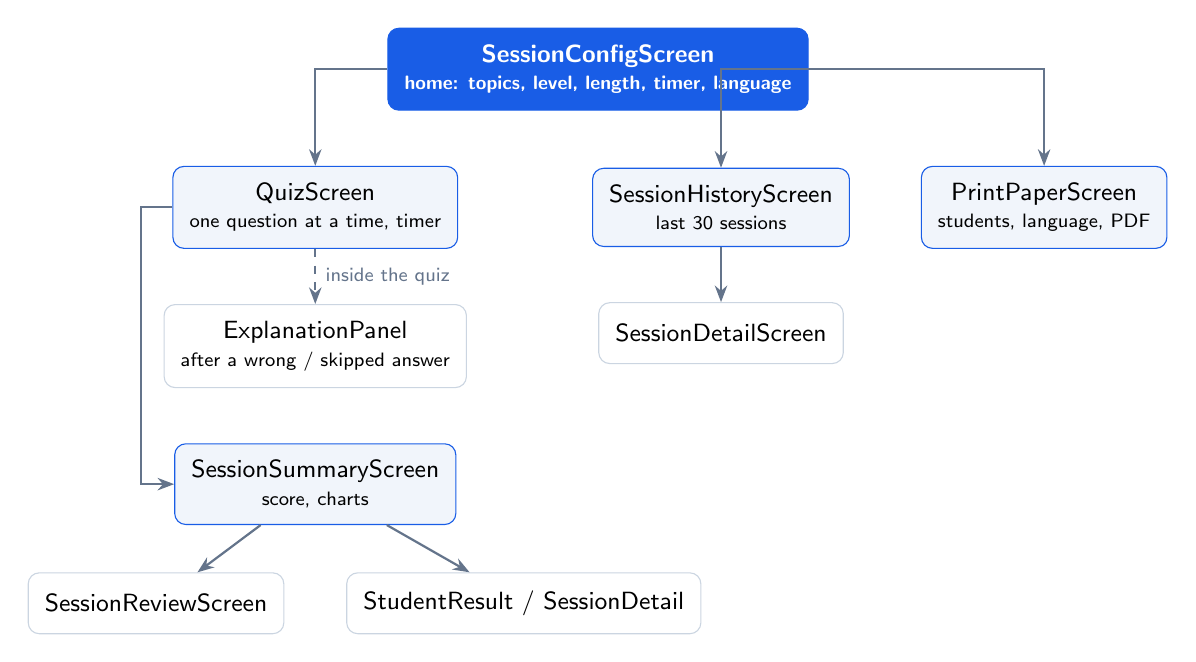
\begin{tikzpicture}[node distance=7mm and 9mm]
  \node[hot] (cfg) {SessionConfigScreen\\[-1pt]{\scriptsize home: topics, level, length, timer, language}};
  \node[box, below left=of cfg, xshift=18mm] (quiz) {QuizScreen\\[-1pt]{\scriptsize one question at a time, timer}};
  \node[plain, below=of quiz] (expl) {ExplanationPanel\\[-1pt]{\scriptsize after a wrong / skipped answer}};
  \node[box, right=of quiz, xshift=8mm] (hist) {SessionHistoryScreen\\[-1pt]{\scriptsize last 30 sessions}};
  \node[box, right=of hist] (print) {PrintPaperScreen\\[-1pt]{\scriptsize students, language, PDF}};
  \node[box, below=of expl] (sum) {SessionSummaryScreen\\[-1pt]{\scriptsize score, charts}};
  \node[plain, below left=6mm and -14mm of sum] (rev) {SessionReviewScreen};
  \node[plain, below right=6mm and -14mm of sum] (det) {StudentResult / SessionDetail};
  \node[plain, below=of hist] (det2) {SessionDetailScreen};
  \draw[flow] (cfg) -| (quiz);
  \draw[flow] (cfg) -| (hist);
  \draw[flow] (cfg) -| (print);
  \draw[flow, dashed] (quiz) -- node[lab, right] {inside the quiz} (expl);
  \draw[flow] (quiz.west) -- ++(-4mm,0) |- (sum.west);
  \draw[flow] (sum) -- (rev);
  \draw[flow] (sum) -- (det);
  \draw[flow] (hist) -- (det2);
\end{tikzpicture}
\caption{Screens. Session lengths: 5, 10, 15, 20, 25, 30, 40 or 50 questions. Timer per question: 30\,s, 1\,min, 2\,min or unlimited.}
\end{figure}

\begin{important}
Read \code{docs/hard-mode-history.md} before changing \code{hard_question_generator.dart} or \code{sandia_painter.dart}. It records about 25 bugs found and fixed there; several look like new reports but had different causes.
\end{important}

\subsection{Code map (\texttt{lib/})}

About 20,000 lines of Dart. The biggest and most important files are in \code{engine/}.

\begin{tbl}{P{0.36\linewidth}L}
\thead{Folder / file} & \thead{What it holds} \\ \midrule
\code{main.dart} & App entry: starts Hive, sets the theme, opens the config screen \\
\code{config/localization.dart} & Every on-screen string in English, Marathi and Hindi (\code{AppLocale.s('key')}); \code{AppLocale.topicName} gives one name per topic for every screen \\
\code{config/version.dart} & Version and build number shown in the app (kept in step with \code{pubspec.yaml} by the release hook) \\
\code{data/} & Hive storage of finished sessions (\code{hive_service.dart}, \code{session_record.dart}; \code{.g.dart} is generated code) \\
\code{engine/question_generator.dart} & \textbf{The router.} \code{QuestionGenerator.generate(topic, difficulty:)} decides which generator makes each question; it also holds the original (``classic'') generators for every topic and stops repeats within a session \\
\code{engine/hard_question_generator.dart} & The \textbf{Sandia engine}: multi-layer shaded matrix questions for Odd Man, Figure Match, Pattern (and Series/Analogy at Hard) \\
\code{engine/exam_style_generator.dart} & Exam-style items copied from real JNVST papers: Geo grid cut, Embedded line drawings, 2$\times$2 Pattern quarters, Figure Match, mirror-image Odd Man, Punch Hole fold sequences, Mirror line figures \\
\code{engine/series_generator.dart}, \code{analogy_generator.dart} & Exam-style Figure Series and Analogy rule families \\
\code{engine/space_vis_generator.dart} & Space Visualisation (which figure the pieces make) \\
\code{engine/book_generator.dart} & Types from the Arihant JNV guide book: letter-word odd man, symbol counting, shifting letters, symbols round a box, paper folding \\
\code{engine/line_figure.dart} & \textbf{\code{LineFig}}: figures as lines on a small grid. Exact turning, flipping, ``is this hidden inside that'', and \code{key} (``do these two look the same as drawn'') \\
\code{engine/test_paper.dart} & Builds a 40-question printed paper and per-student shuffled sets \\
\code{engine/difficulty.dart} & \code{Difficulty \{ easy, medium, hard \}} \\
\code{engine/explanation.dart} & \textbf{Answer explanations.} \code{Explanation.of(question)} works out what to animate for any question (or \code{null}), once per question \\
\code{engine/explain/} & One file per topic group (\code{pattern}, \code{series}, \code{analogy}, \code{odd_man}, \code{figure_match}, \code{geo}, \code{space_vis}) that turns a question into a \code{Scene} \\
\code{engine/scene.dart} & The \code{Scene} model: slots (figures placed on a small stage) and steps (fly, morph, pulse, tick, reveal) \\
\code{engine/morph.dart}, \code{morph_line.dart} & Work out the difference between two figures as ``beats'' (turn, flip, resize, move, swap) and draw any in-between frame \\
\code{engine/paper_fold.dart} & Unfolds punched paper one fold at a time for the Punch Hole explanation \\
\code{painters/} & Code that draws each figure type: \code{line_figure_painter} (LineFig), \code{sandia_painter} (shaded matrices), \code{figure_painter} (classic shapes), \code{mirror_text_painter}, \code{punch_painter}, \code{geo_piece_path} \\
\code{widgets/question_renderer.dart} & Draws the question area for each puzzle type \\
\code{widgets/option_renderer.dart} & Draws each answer option; picks the painter from the option's \code{type} \\
\code{widgets/explanation_panel.dart}, \code{scene_player.dart} & Play an explanation: the panel runs the timer and Replay button; the scene player draws a \code{Scene} at any point of its timeline \\
\code{paper/paper_pages.dart}, \code{paper_pdf.dart} & Layout and PDF output of printed papers \\
\code{screens/} & The screens shown above \\
\end{tbl}

\subsection{How a question is stored}

Every question is a \code{ReasoningQuestion}: a topic, a type name (e.g.\ \code{geo_grid_cut}), a \code{puzzle} map describing the question figure, four \code{options} maps, and \code{correctIndex}. Maps are plain data, so they can be saved, compared, tested and drawn anywhere. The \code{type} inside each map tells the renderer which painter to use:

\begin{tbl}{P{0.28\linewidth}P{0.3\linewidth}L}
\thead{\texttt{type}} & \thead{Drawn by} & \thead{Used for} \\ \midrule
\code{line_fig} & \code{LineFigurePainter} & Most exam-style figures (grid of lines, black half-cells, dots, arrows, hatching, arcs, symbols) \\
\code{sandia_cell} & \code{SandiaPainter} & Shaded multi-shape matrix cells (Hard engine) \\
(no type: \code{shape}, \code{rotation}, \code{dots}\dots) & \code{EnhancedFigurePainter} & Classic single-shape figures \\
\code{mirror_text} & \code{EnhancedMirrorTextPainter} / \code{MirrorTextPainter} & Letters, digits, clocks \\
\code{punch_hole} & \code{PunchPainter} & Punched paper \\
\code{geo_piece} & geometry piece painters & Classic Geo Completion \\
\end{tbl}

% ================================================================ 5
\section{How questions are made}

\subsection{The routing rule}

\code{QuestionGenerator.generate(topic, difficulty:)} picks a generator by topic and level, often by a weighted coin toss. For example, Medium Figure Series is about 60\% exam-style series, 20\% guide-book series and 20\% classic series. The full mix is in \code{_generateMediumRaw} (Medium) and \code{_generateRaw} (Easy and Hard) in \code{question_generator.dart}.

\subsection{Design rules every generator follows}

These rules came out of real bug reports (section~\ref{sec:problems}). Keep them when adding questions.

\begin{enumerate}
\item \textbf{Add, never replace.} New generators are added to a topic's mix; the old ones stay. The mentors asked for variety, and old generators are tested.
\item \textbf{One right answer, by construction and by test.} Every generator works out the answer from its own rule, and a test re-solves the question from the drawings alone and checks exactly one option fits.
\item \textbf{``Looks the same'' means as drawn.} Two options are different only if a person can see the difference. \code{LineFig.key} ignores lines hidden on a black edge or the frame and dots hidden on a line; the Sandia engine renders options on a 64$\times$64 grid and requires 5\% of the cell to change by 50/255.
\item \textbf{Nothing hidden.} No figure may contain a detail you can't see (e.g.\ a dot under a black triangle) -- \code{LineFig.hasHiddenDetail}.
\item \textbf{Balanced wrong options.} The four options form a balanced set (e.g.\ \{right change, wrong change\} $\times$ \{right count, wrong count\}) so the answer is never ``the odd one out'' of the options or ``the one in the middle''. Tests check no option is uniquely central.
\item \textbf{No flipped copies where a flip is legal.} A cut-out Geo piece can be turned over, so no option may be the answer flipped. An Embedded wrong option may not hide the shape in any orientation.
\item \textbf{Level meaning.} Easy changes one thing per question (grades 2--3). Medium is a true midpoint, never Easy or Hard material. Hard is exam level.
\end{enumerate}

\subsection{Adding a new question type (recipe)}

\begin{enumerate}
\item Write a generator that returns \code{ReasoningQuestion?} (return \code{null} if a random draw fails a check; the router falls back).
\item Use an existing figure \code{type} (usually \code{line_fig}) so no new painter is needed.
\item Shuffle the options and record \code{correctIndex}.
\item Add it to the router at a small share for the right levels.
\item Write a test that solves the question from its data and checks exactly one option is right (see \code{test/book_generator_test.dart} for small examples).
\item Run \code{flutter test}; the cross-topic tests (\code{no_hidden_detail_test}, \code{question_generator_test}, visual tests, \code{explanation_all_topics_test}) will also check it.
\item Check the new type gets an explanation (\ref{sec:explanations}). Most \code{line_fig} and Sandia types are explained automatically; if \code{explanation_all_topics_test} lists the new type as unexplained, add it to the topic's file in \code{engine/explain/}.
\end{enumerate}

\subsection{Answer explanations}\label{sec:explanations}

After a wrong, skipped or timed-out answer, an \textbf{ExplanationPanel} appears under the result. It plays a short animation (3--6.5\,s) on the question's own figures, ending on the correct option framed in green. It has no words, so it works the same in all three languages. \textbf{Next} stays locked until it finishes; \textbf{Replay} (\faRedo) plays it again. If the phone has ``remove animations'' switched on, the panel shows the final frame.

Explanations are \textbf{worked out from the question data}, not stored with the question. That is why sessions saved before explanations existed have them too. \code{Explanation.of(q)} returns \code{null} for anything it can't explain; the quiz then simply shows no panel, so a gap is never a crash.

\begin{figure}[H]
\centering
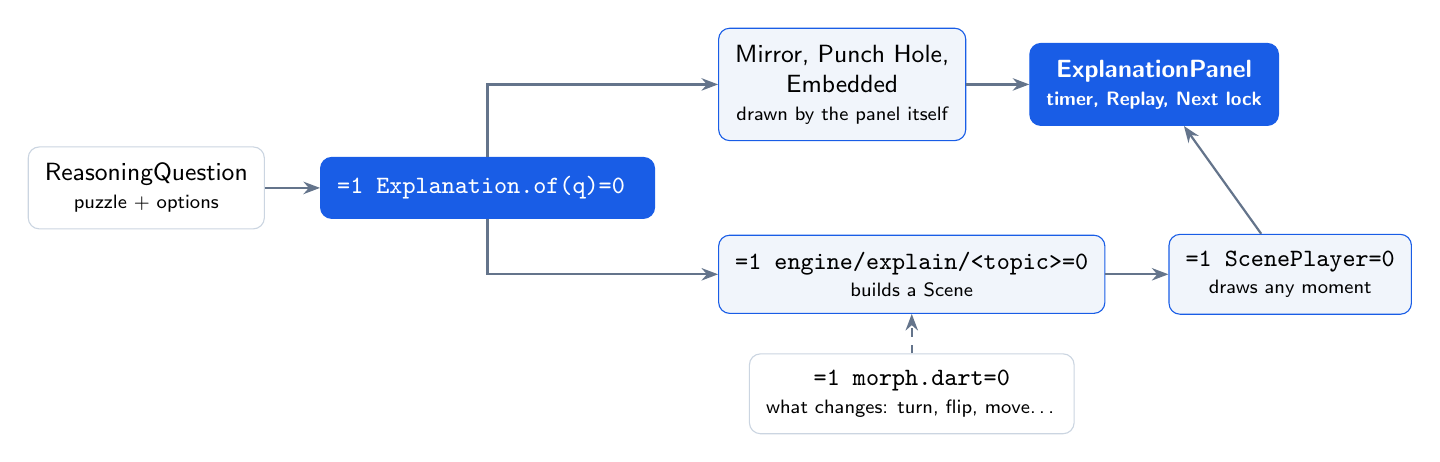
\begin{tikzpicture}[node distance=5mm and 7mm]
  \node[plain] (q) {ReasoningQuestion\\[-1pt]{\scriptsize puzzle + options}};
  \node[hot, right=of q] (of) {\code{Explanation.of(q)}};
  \node[box, above right=2mm and 8mm of of] (direct) {Mirror, Punch Hole,\\Embedded\\[-1pt]{\scriptsize drawn by the panel itself}};
  \node[box, below right=2mm and 8mm of of] (scene) {\code{engine/explain/<topic>}\\[-1pt]{\scriptsize builds a Scene}};
  \node[plain, below=of scene] (morph) {\code{morph.dart}\\[-1pt]{\scriptsize what changes: turn, flip, move\dots}};
  \node[box, right=8mm of scene] (player) {\code{ScenePlayer}\\[-1pt]{\scriptsize draws any moment}};
  \node[hot, right=8mm of direct] (panel) {ExplanationPanel\\[-1pt]{\scriptsize timer, Replay, Next lock}};
  \draw[flow] (q) -- (of);
  \draw[flow] (of) |- (direct);
  \draw[flow] (of) |- (scene);
  \draw[flow, dashed] (morph) -- (scene);
  \draw[flow] (scene) -- (player);
  \draw[flow] (player) -- (panel);
  \draw[flow] (direct) -- (panel);
\end{tikzpicture}
\caption{How an explanation is made. \code{null} at any point means ``no panel''.}
\end{figure}

\subsubsection*{What each topic shows}

\begin{tbl}{P{0.24\linewidth}L}
\thead{Topic} & \thead{What the animation shows} \\ \midrule
Mirror Shape / Text & The figure flips over the mirror line onto the answer \\
Punch Hole & The punched paper unfolds fold by fold (last fold first); paper folding: the sheet's half folds over \\
Embedded & The hidden shape lights up inside the answer \\
Figure Series & Each frame flies to the next, changing the same way every step; the last flies into the ``?'' (frames wrap onto two rows on small phones) \\
Analogy & A copy of A flies onto B, changing on the way; a copy of C makes the same changes and lands in the ``?'' \\
Pattern & The row/column rule is shown on two example cells, then applied in the gap. Sandia grids are built \textbf{layer by layer}, because each layer (and each part, e.g.\ shape vs shading) can follow its own line \\
Odd Man Out & What the three alike options share is shown (turned copies fly onto each other until they match); the odd one is outlined in red \\
Figure Match & A copy of the target flies onto the correct option, turning or flipping on the way, and covers it exactly \\
Geo Completion & The correct piece turns the right way up and slides into the gap; the completed shape glows \\
Space Visualisation & The answer is cut into regions; each given piece turns or flips to match its region and flies into place \\
\end{tbl}

\subsubsection*{What they look like}

Each strip below is one real explanation from the app, captured at four moments: the start (left), two moments in between, and the end with the correct option framed in green (right).

\filmstrip{analogy}{Analogy: A turns into B; C makes the same change and lands in the ``?''}
\filmstrip{series}{Figure Series: each frame flies to the next with the same turn}
\filmstrip{pattern}{Pattern (Hard, Sandia): the missing cell is built layer by layer from its neighbours}
\filmstrip{punch}{Punch Hole: the paper unfolds fold by fold}
\filmstrip{mirror}{Mirror Shape: the figure flips over the mirror line}
\filmstrip{odd_man}{Odd Man Out: what the alike options share, and the odd one}
\filmstrip{geo}{Geo Completion: the piece turns and slides into the gap}
\filmstrip{space_vis}{Space Visualisation: each piece turns to fit its region}

\subsubsection*{Tests}
\code{explain_<topic>_test.dart} generate hundreds of questions per type and check that each scene really ends on the correct option and that each step shows the real rule (for example, the example cells in a Pattern scene change by the same amount as the gap). \code{explanation_all_topics_test} checks every question type has an explanation.

\subsubsection*{Known limits (beta 9)}
\begin{itemize}
\item A few Hard Pattern grids (2 in the test run) still show only the change, not a rule: one Sandia grid where the grid itself doesn't decide the answer (a generator flaw, see \ref{sec:open}), and one dual-rule grid where the dots stop at 4.
\item A shape that spins and lands looking the same (a symmetric shape) still spins: the spin shows the rule's turn, and this was kept on purpose.
\end{itemize}

% ================================================================ 6
\section{The printed test paper}

Coordinators open \textbf{Print paper} on the config screen (the \faPrint\ button), choose the number of students (1--60) and the \textbf{paper language} (English, Marathi, or both), and press \textbf{Make PDF}. Android's print/share dialog opens with the PDF.

\begin{figure}[H]
\centering
\begin{minipage}[b]{0.27\linewidth}\centering\phone[0.26]{screen_print}\end{minipage}\hfill
\begin{minipage}[b]{0.66\linewidth}\centering
\tcbox[enhanced,colback=white,colframe=rule,boxrule=0.6pt,arc=2pt,left=0pt,right=0pt,top=0pt,bottom=0pt,drop fuzzy shadow]{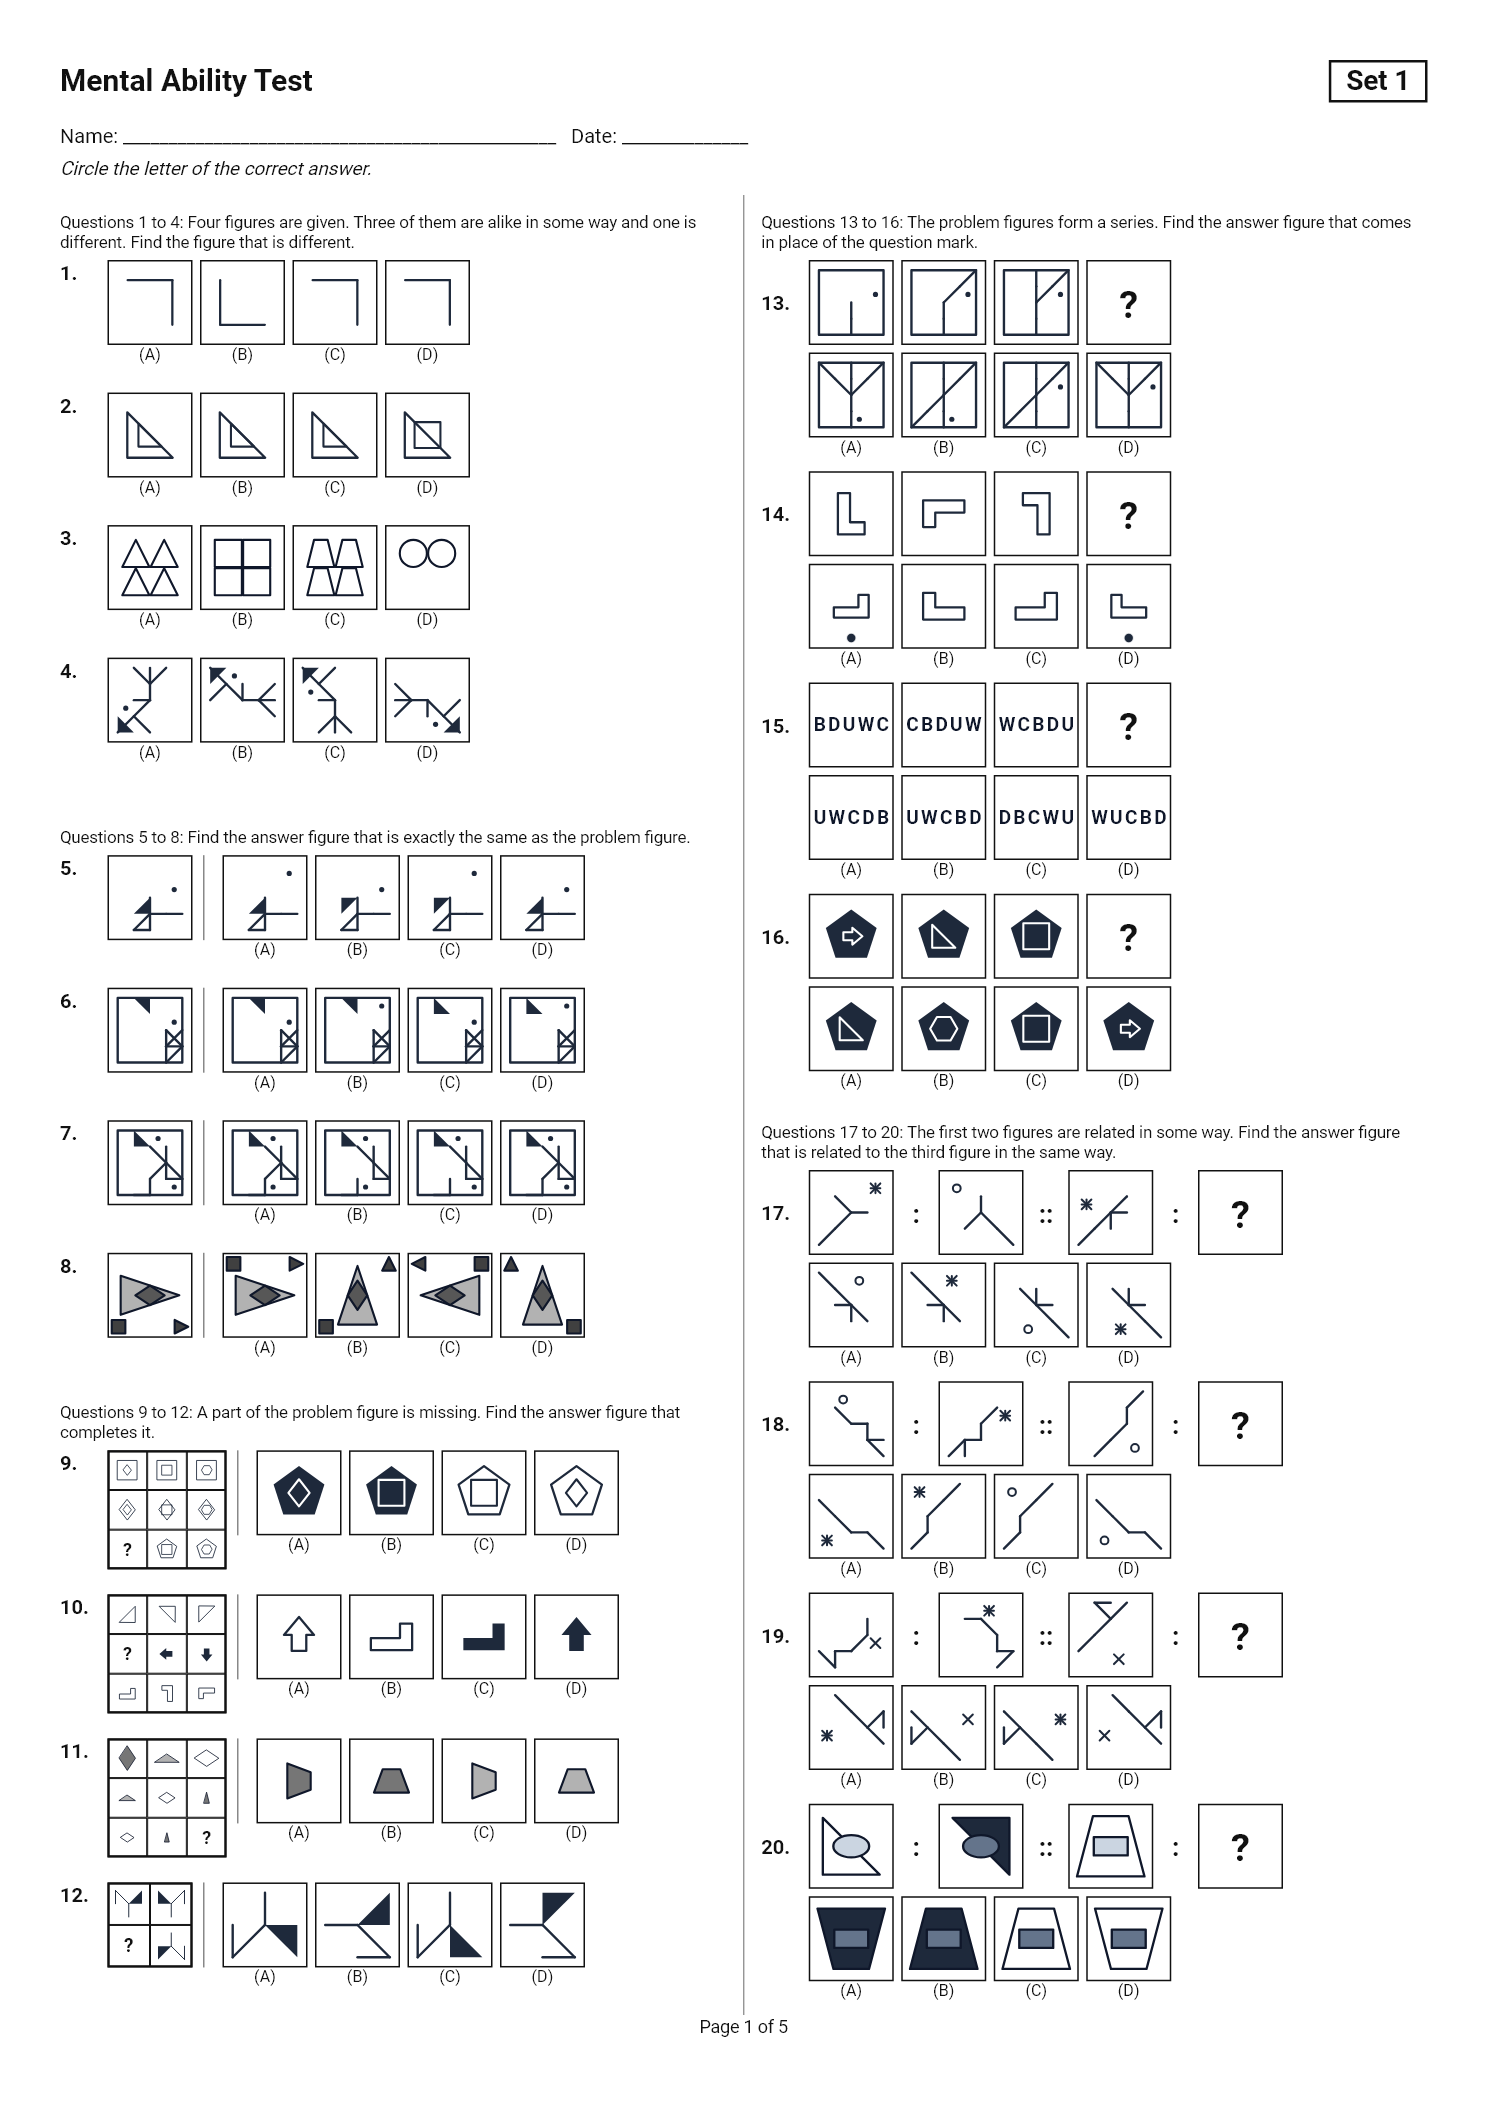
\includegraphics[width=0.96\linewidth]{paper_side1}}
\end{minipage}
\caption{Left: the Print paper screen. Right: side 1 of a student's paper -- 20 questions in two columns, in JNVST part order.}
\end{figure}

\begin{tbl}{P{0.22\linewidth}L}
\thead{Feature} & \thead{How it works} \\ \midrule
Content & 10 parts $\times$ 4 questions in JNVST order (\code{TestPaper.partIds}) \\
Difficulty per part & \code{TestPaper.partLevels}: mostly 1 Easy, 2 Medium, 1 Hard; Odd Man, Figure Match, Geo have no Easy; Analogy 3 Medium + 1 Hard (mentors' request) \\
Per-student sets & Same 40 questions, shuffled within equal-difficulty runs, options shuffled; teacher key on the last page \\
Layout & A4, 20 questions a side in two columns, exam style: single-figure questions on one line, series/analogy/folding on two lines. Figures 10--14\,mm, 3$\times$3 grids 1.4$\times$ bigger \\
Drawing & Pages are drawn by the app's own painters at app size (80\,px) then scaled down, so lines keep their proportions; converted to grayscale and compressed (\code{_grayPage}, about 0.3\,s a page) \\
Languages & \code{paperText(langs, key)}; with both languages the directions print English then Marathi \\
\end{tbl}

\code{paper_pdf.dart} uses one internal file of the \code{pdf} package (\code{package:pdf/src/pdf/format/num.dart}) to add pre-compressed images. If \code{pdf} is upgraded past 3.12 and this breaks, see \ref{sec:upgrades}.

% ================================================================ 7
\section{How we work: testing, feedback, releases}

\subsection{Testing method}

The project relies on automated tests because a person can't check thousands of generated questions by eye. There are 47 test files and 365 tests. The main kinds:

\begin{tbl}{P{0.18\linewidth}P{0.4\linewidth}L}
\thead{Kind} & \thead{Example files} & \thead{What they prove} \\ \midrule
Solve-from-data & \code{series_test}, \code{analogy_test}, \code{space_vis_test}, \code{book_generator_test}, \code{exam_style_test} & Hundreds of questions per type; each is solved from its drawings and exactly one option is right \\
Level properties & \code{easy_level_test}, \code{medium_level_test} & Easy changes one thing; Medium is between Easy and Hard \\
Look-alike / visibility & \code{line_figure_key_test}, \code{no_hidden_detail_test}, \code{question_generator_visual_dedup_test}, \code{hard_generator_visual_test}, \code{sandia_outline_test} & No two options look the same when drawn; nothing hidden \\
Engine diagnostics & \code{hard_generator_diagnostics_test} & Sandia engine: no crashes, no duplicates, no tiny features \\
Screens & \code{quiz_layout_test}, \code{multi_topic_test}, \code{report_screens_test}, \code{print_paper_screen_test} & Screens build and behave at phone size \\
Paper & \code{paper_pdf_test}, \code{test_paper_test}, \code{mentor_paper_review_test} & Every page fits A4 in all languages; PDF page counts; mentors' review points \\
Explanations & \code{explain_*_test}, \code{explanation_test}, \code{morph_test}, \code{scene_player_test}, \code{explanation_panel_test}, \code{explanation_quiz_test} & Every animation ends on the correct option and shows the real rule; frames draw without errors; the quiz locks Next until it ends \\
\end{tbl}

\begin{tip}
Every bug fix starts with a test that fails; the fix then makes it pass. This rule kept the same bugs from coming back.
\end{tip}

\subsection{Feedback loop}

\begin{figure}[H]
\centering
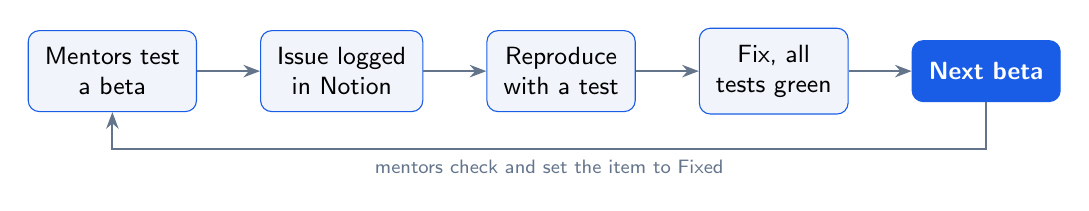
\begin{tikzpicture}[node distance=8mm]
  \node[box] (a) {Mentors test\\a beta};
  \node[box, right=of a] (b) {Issue logged\\in Notion};
  \node[box, right=of b] (c) {Reproduce\\with a test};
  \node[box, right=of c] (d) {Fix, all\\tests green};
  \node[hot, right=of d] (e) {Next beta};
  \draw[flow] (a) -- (b); \draw[flow] (b) -- (c); \draw[flow] (c) -- (d); \draw[flow] (d) -- (e);
  \draw[flow] (e.south) -- ++(0,-6mm) -| node[lab, pos=0.25, below] {mentors check and set the item to Fixed} (a.south);
\end{tikzpicture}
\end{figure}

\begin{enumerate}
\item Mentors test a beta on their phones and log each issue in the \textbf{Notion tracker} (Name, Bug/Feature, Status, screenshots in the comments).
\item The developer reads the tracker (the developer never edits it -- the mentors own it), reproduces the problem with a test, fixes it, and reports back.
\item Fixes are released as the next beta; the mentors set the item to \textbf{Fixed} after checking.
\end{enumerate}
Printed papers were reviewed the same way, by WhatsApp messages and PDF annotations from the mentors.

\subsection{Git branches}\label{sec:branches}

\begin{tbl}{P{0.3\linewidth}L}
\thead{Branch} & \thead{Role} \\ \midrule
\code{master} & Release line. Every beta is tagged on master. \\
\code{hard-mode-exam-style} & Where all work since September 2026 was done, including answer explanations; merged into master for each release (last: beta 9) \\
\code{session-rework} & Older main work branch. It does \textbf{not} have the work since beta 8 (explanations); treat master as the source of truth \\
\code{generator-rework}, \code{generator-revamp}, \dots & Older feature branches, already merged \\
\code{release-check} & Local-only branch used to test the beta 8 merge; can be deleted \\
\end{tbl}

Work on a branch, run \code{flutter analyze} and \code{flutter test}, then merge into master for a release.

\subsection{Making a beta release}

Version format: \code{pubspec.yaml} \code{version: 1.0.0-beta.N+N}, tag \code{v1.0.0-beta.N}. \code{lib/config/version.dart} must match (\code{preRelease = 'beta.N'}, \code{buildNumber = N}).

\begin{figure}[H]
\centering
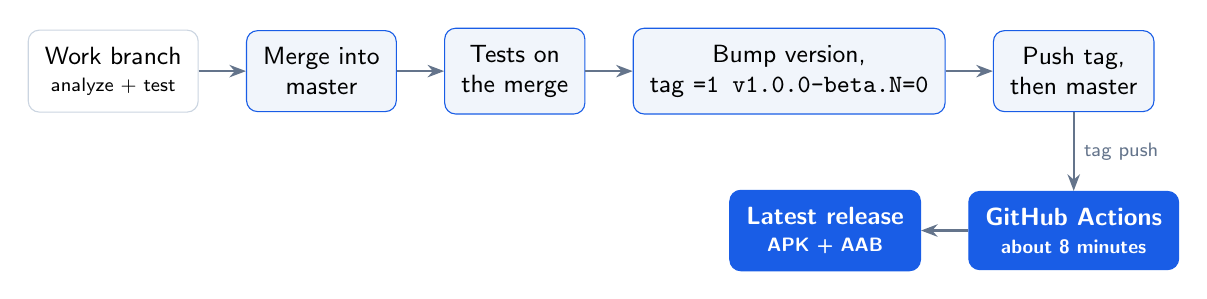
\begin{tikzpicture}[node distance=6mm]
  \node[plain] (w) {Work branch\\[-1pt]{\scriptsize analyze + test}};
  \node[box, right=of w] (m) {Merge into\\master};
  \node[box, right=of m] (t) {Tests on\\the merge};
  \node[box, right=of t] (v) {Bump version,\\tag \code{v1.0.0-beta.N}};
  \node[box, right=of v] (p) {Push tag,\\then master};
  \node[hot, below=10mm of p] (ci) {GitHub Actions\\[-1pt]{\scriptsize about 8 minutes}};
  \node[hot, left=of ci] (r) {Latest release\\[-1pt]{\scriptsize APK + AAB}};
  \draw[flow] (w) -- (m); \draw[flow] (m) -- (t); \draw[flow] (t) -- (v); \draw[flow] (v) -- (p);
  \draw[flow] (p) -- node[lab, right] {tag push} (ci); \draw[flow] (ci) -- (r);
\end{tikzpicture}
\end{figure}

\begin{enumerate}
\item Merge the work branch into \code{master}; resolve conflicts; run \code{flutter analyze} and \code{flutter test} on the result.
\item Push master: \code{git push origin master}.
\item The \textbf{pre-push hook} (\code{tools/git-hooks/pre-push}) asks ``cut a new beta?'' -- in a dialog box on Windows, a zenity dialog on a Linux desktop, or as a question in the terminal otherwise. Click \textbf{Yes} and accept the suggested tag. It bumps both version files, commits, tags and pushes the tag. (If you made the version commit and tag yourself, click \textbf{No}.)
\item Pushing the tag starts \textbf{GitHub Actions}: it checks the tag matches \code{pubspec.yaml}, runs analyze and tests, builds the APK and AAB, and publishes them as the \textbf{Latest} release (about 8 minutes). Watch it under the repo's \textbf{Actions} tab or with \code{gh run list}.
\item Send testers the release link. They install \code{app-release.apk} (see \ref{sec:signing} about signing).
\end{enumerate}

\begin{tip}
Beta 9 was released the manual way, which avoids one quirk of the hook (its version commit is made after git has decided what to push, so master can end up one commit behind the tag until the next push). Manual steps: bump \code{pubspec.yaml} and \code{version.dart}, commit, \code{git tag -a v1.0.0-beta.N -m "..."}, \code{git push origin v1.0.0-beta.N}, then \code{git push origin master} and click \textbf{No} in the hook's dialog.
\end{tip}

\begin{important}
Never delete or reuse a published tag. If something is wrong, fix it and release the next beta number (\code{docs/release_beta.md}).
\end{important}

% ================================================================ 8
\section{History: how the project grew}

\begin{tbl}{P{0.14\linewidth}L}
\thead{When (2026)} & \thead{Milestone} \\ \midrule
Jan--Mar & Project started; quiz engine, sessions, review screen. Switched from static image questions to \textbf{generated questions} drawn by code. \\
Mar--Apr & Intelligent Bias, weak-area practice, Hive history, Marathi then Hindi, session detail and student result screens \\
May & First betas (beta 1--3); automated version tracking; Mirror Text overhaul; Java/Gradle CI fixes \\
Jul--Aug & \textbf{Hard Mode} with the Sandia matrix engine (shaded multi-layer figures based on the Sandia Generated Matrix Tool); beta 4; pre-push release hook \\
Sep & Exam-style questions from real JNVST papers for every topic; Space Visualisation topic; LineFig drawing parts (arrows, hatching, arcs, symbols); multi-topic sessions; \textbf{Medium} level; beta 5--6 \\
Oct & Medium reworked as a true midpoint; \textbf{printed test paper} (A4 PDF, per-student sets); guide-book question types; English/Marathi papers; many fixes from mentors' reviews; beta 7 \\
3 Nov & \textbf{Beta 8}: everything above plus all tracker fixes \\
4 Nov & \textbf{Beta 9}: answer explanations for all 11 topics (animated, wordless), Sandia Pattern grids explained layer by layer, series frames on two rows for small phones \\
\end{tbl}

The full list of commits is in \code{git log}; Hard Mode decisions are written up in detail in \code{docs/hard-mode-history.md}; \code{CHANGELOG.md} covers the early betas.

% ================================================================ 9
\section{Problems we hit and how we fixed them}\label{sec:problems}

Grouped by area. For each: what went wrong, the real cause, and the fix. The same kinds of problems tend to come back, so section~\ref{sec:troubleshooting} turns these into a checklist.

\newcommand{\probhead}{\thead{Problem} & \thead{Cause} & \thead{Fix} \\ \midrule}
\newcolumntype{Q}{P{0.3\linewidth}P{0.31\linewidth}L}

\subsection{Questions with two right answers or look-alike options}

The most common class of bug. It almost always had the same shape: two options that differ in the data but \textbf{look} the same on screen.

\begin{tbl}{Q}\probhead
Hard Pattern/Odd Man options came in ``two identical pairs'' & Wrong options are built from two changes in every combination; if one change was invisible, options paired up & Every Sandia question is rendered on a 64$\times$64 grid and rejected if any two options differ too little (\code{_hasNearDuplicateOptions}, hard-mode-history \#14--17) \\
Shaded options still looked alike to testers (Oct 2026) & The visibility bar (2\% of the cell, 30/255) let dark-on-dark changes through & Raised to 5\% of the cell and 50/255 (\#25). Near-twin pairs in Figure Match Hard went from 32/84 to 0 \\
Pattern 2$\times$2 options A and C identical & A changed line ran exactly along a black triangle's edge, so it couldn't be seen & \code{LineFig.key} treats lines on black edges and on the frame as invisible \\
Figure Match duplicates (tracker, Oct) & A dot drawn on a diagonal line or a black half-cell disappears & \code{key} ignores hidden dots; generators reject any figure with a hidden dot (\code{hasHiddenDetail}) \\
Geo Completion: two pieces fit (mentors, Oct) & A wrong piece was the answer \textbf{flipped over}; a paper piece can be turned over & Pieces are compared up to turning \textbf{and} flipping (\code{flipClass}); wrong pieces are one-cell changes only \\
Embedded Figure: a wrong option ``contained'' the shape (testers) & Wrong options hid the shape turned or flipped, which children read as ``it's there'' & Wrong options hide a near-miss shape (one stroke moved) and never the shape in any orientation \\
2$\times$2 Pattern: options differ only by a dot & The ``small change'' moved a dot one cell & The wrong option's change is the black half-cell flipping instead \\
Odd Man (Sandia) rotations identical for rectangle/diamond & Shapes symmetric under 180° look the same at 0° and 180° & Comparison knows each shape's symmetry; orientations spread over 180° \\
Series/Analogy duplicates from a cross background & The cross looks the same every 90° & Removed symmetric backgrounds from the pools \\
\end{tbl}

\subsection{Questions that were too hard, too easy or unclear}

\begin{tbl}{Q}\probhead
Easy questions too hard for grades 2--3 & Easy reused Hard-style multi-change rules & Easy changes one thing per question in every topic; tests pin it \\
Medium was ``Easy or Hard by coin toss'' & First Medium version mixed the two & Medium got its own router with lite settings of each generator \\
Mentors: paper questions 1--6, 8, 17, 21--23 too easy (facilitators also sit it) & Paper used Easy/Easy/Medium/Medium & Per-topic mix with Hard questions \\
Series showed 4 figures before the ``?'' & One series type (\code{series_alt_dual}) used 4 frames & Every series shows 3 figures then ``?'' \\
Punch Hole folds unclear on paper & No direction shown & Fold arrows on every fold panel \\
Mirror Text level mismatch (tracker) & One length for every level & Easy 1--2 characters, Medium 2--3, Hard 4 \\
Session title said ``Mirror image'' for both mirror topics (tracker) & Separate, older title strings & One \code{AppLocale.topicName} for config and session \\
\end{tbl}

\subsection{Drawing problems}

\begin{tbl}{Q}\probhead
Question figure looked different from its own correct option & Question area used an older painter & The question area draws with the same code as the options \\
Detail on filled shapes vanished & Dark details on dark fills & White details with a navy outline \\
White diamond on a black rectangle invisible & Dark outline on dark fill & Outlines drawn after a dark shape get a white edge \\
Mirror Text distorted / numbers mirrored wrongly & Text mirrored on the canvas directly & Text drawn to a picture first, then mirrored \\
Letters showed as black blocks in test renders & Flutter tests use a block font unless a font is named & Letter painters name Roboto (Android's default) \\
L shape's mirror and turn looked alike & Foot and upright too similar in length & Foot 1.1 vs upright 1.7 units; pixel test \\
\end{tbl}

\subsection{Printed paper problems}

\begin{tbl}{Q}\probhead
Too few questions per page (coordinator wanted 20 a side) & One question per row & Two columns, exam style, flow down then across \\
Figures dense on paper (lines swamp details) & Painters use fixed 2--3\,px lines tuned for 80\,px figures; paper boxes are 13\,mm & Draw at 80\,px and scale down; no inner Sandia frame in print \\
Dots touching the box & Classic figures put dots near the bottom edge & Small margin around classic figures in print \\
PDF slow (1.3--2\,s a page) & PNG encode/decode in Dart & Grayscale + zlib compression directly (0.3\,s a page) \\
Marathi wanted & English only & Language picker: English, Marathi, both \\
Shading may vanish on a photocopier & Light greys become white in pure black/white copies & Not changed yet -- see \ref{sec:open} \\
\end{tbl}

\subsection{Build, CI and tooling problems}\label{sec:buildproblems}

\begin{tbl}{Q}\probhead
CI failed with a Java toolchain error & Gradle daemon JVM settings pointed at a local Java & CI uses Temurin 17 and deletes \code{gradle-daemon-jvm.properties} before building \\
Gradle / Android Gradle Plugin mismatch & Upgrading Gradle to 9.x broke the Flutter Gradle plugin & Pinned Gradle 8.14.3 with AGP 8.13.0 (Flutter doesn't support AGP 9 yet) \\
Beta 6 CI failed & Tests depended on a Windows-only font & Tests no longer load Windows fonts \\
pubspec version and in-app version drifted & Two files updated by hand & The pre-push hook updates both together \\
Hook suggested the wrong next beta & It didn't notice an untagged version & Fixed in the hook (Sep) \\
Release hook blocked pushes on Linux & It called Windows-only \code{powershell.exe} & The hook picks Windows dialogs, zenity, or terminal prompts automatically (Nov) \\
Debug and release app couldn't both be installed & Same package name & Debug builds use the \code{.debug} suffix \\
Releases didn't show on the GitHub repo page & Published as pre-releases & Published as Latest releases \\
\code{INSTALL_FAILED_UPDATE_INCOMPATIBLE} on the phone & Release builds are signed with a CI-generated debug key that changes each run & Uninstall then install; permanent fix in \ref{sec:signing} \\
\end{tbl}

\subsection{Answer explanation problems}

\begin{tbl}{Q}\probhead
No explanation showed on the phone for any topic & The tester was running the beta (release) app, not the newly installed debug app; they sit side by side & Open the app whose package ends in \code{.debug} (section 3) \\
Debug app showed an old version (``beta 5'') & The work branch's \code{version.dart} hadn't been updated with master's releases & Keep \code{pubspec.yaml} and \code{version.dart} in step on the work branch too \\
Hard Pattern explanations showed only the difference, not the rule, for almost every Sandia grid (94 in the test run) & Each Sandia layer, and each part of a layer, follows its own line through the grid; a single row/column rule doesn't exist & Explanations build the answer layer by layer, each from its own line, with a two-cell example first \\
A shade change ``by 0'' counted as a change & Equal values were compared as different & Shade changes need different values; tests mirror the check \\
The frame around an arrow swung into a diamond mid-turn & The whole figure, frame included, was turned & Square frames are drawn still; only what is inside turns \\
The copy landed on a grey ``?'' box & The question box stayed visible under the flying figure & The ``?'' fades out as the copy arrives \\
Series frames shrank to fit a 360\,dp phone & All frames on one row & Two rows when one row would shrink them \\
\end{tbl}

\subsection{Process problems}

\begin{tbl}{Q}\probhead
A whole feature (Medium) had to be reverted before beta 6, then restored for beta 7 & It wasn't ready when the release was cut & Release only from a branch that passes all tests; trial-merge first \\
A history doc once described fixes that weren't in the code & Notes written from memory & Every fix now has a test; trust tests over notes \\
Testers kept reporting bugs that were already fixed & Their phones ran the old beta & Release more often; check which beta a screenshot comes from \\
\end{tbl}

% ================================================================ 10
\section{Troubleshooting future problems}\label{sec:troubleshooting}

\subsection{A tester reports ``two options look the same'' or ``two answers fit''}

\begin{enumerate}
\item \textbf{Find the build.} Ask which beta they run (the version badge on the home screen shows it, e.g.\ ``v1.0.0-beta.9 Damson''). If it's older than the latest, ask them to update first.
\item \textbf{Find the generator.} The topic is in the screenshot header; the question type tells you the file (section~4.3). Run a quick script or test that generates that topic and level and prints \code{q.type} to narrow it down.
\item \textbf{Reproduce with a test.} Generate a few hundred questions of that type and check the property that failed (e.g.\ ``no two options have the same \code{key}'', ``only one option embeds the target'').
\item \textbf{Look for the usual causes:} something hidden (on a line, a black area or the frame); a flip or turn being legal for the solver; a shape that is symmetric so a turn changes nothing; a visibility bar too low.
\item \textbf{Fix in the generator} (reject such draws or change the wrong-option rule), not in the painter, unless the drawing itself is wrong.
\item Run the full test suite, install a debug build, check on the phone.
\end{enumerate}

\subsection{An explanation is missing, wrong or looks odd}

\begin{enumerate}
\item \textbf{Check the app.} Explanations exist from beta 9. On a development phone, make sure you opened the \code{.debug} app if you installed a debug build.
\item \textbf{Find the type.} No panel at all means \code{Explanation.of(q)} returned \code{null} for that question type (it never crashes; any error inside it also gives \code{null}). \code{explanation_all_topics_test} prints which types have no explanation.
\item \textbf{Reproduce with a test.} In the topic's \code{test/explain_<topic>_test.dart}, generate that type and check the property that's wrong (wrong end frame, a step that doesn't match the rule).
\item \textbf{Fix in \code{engine/explain/<topic>.dart}} (what the scene shows) or \code{morph.dart} (how two figures differ). Drawing glitches mid-animation are usually in \code{scene_player.dart} or a painter's in-between frame handling.
\item If the explanation can't show a rule because the question doesn't have one, the bug is in the \textbf{generator}, not the explanation.
\end{enumerate}

\subsection{The phone isn't found}\label{sec:nophone}

\begin{tbl}{P{0.36\linewidth}L}
\thead{Symptom} & \thead{Fix} \\ \midrule
\code{adb devices} is empty & Turn \textbf{Wireless debugging} back on (it switches off on sleep / network change), or plug in the cable \\
Installed fine but changes don't show & You opened the release (beta) app; the debug build installs as a second app (package ends in \code{.debug}) \\
``more than one device/emulator'' & The phone is listed twice; use \code{adb -s <one-of-the-names> ...} \\
``unauthorized'' & Accept the prompt on the phone; if none, revoke USB debugging authorisations in Developer options and reconnect \\
\code{INSTALL_FAILED_UPDATE_INCOMPATIBLE} & The installed app has a different signature: \code{adb uninstall <package>} then install (this deletes that app's local history) \\
\end{tbl}

\subsection{Build fails}

\begin{tbl}{P{0.36\linewidth}L}
\thead{Symptom} & \thead{Fix} \\ \midrule
Dependency errors after \code{git pull} & \code{flutter clean} then \code{flutter pub get} \\
Gradle/AGP version errors & Keep Gradle 8.14.3 and AGP 8.13.0 (\code{android/gradle/wrapper/gradle-wrapper.properties}, \code{android/settings.gradle.kts}); don't upgrade AGP to 9.x until Flutter supports it \\
Java errors & Use Java 17 or newer; \code{flutter doctor -v} shows which one Flutter uses. To point Flutter at a specific JDK: \code{flutter config --jdk-dir "<path to JDK>"} \\
CI fails at ``Validate tag'' & Tag and \code{pubspec.yaml} version differ; fix \code{pubspec.yaml}, release the next beta number \\
CI fails at ``Test'' but tests pass locally & Look for tests depending on Windows paths or fonts; tests must not use \code{C:\textbackslash{}...} \\
\end{tbl}

\subsection{Tests fail after a change}

\begin{itemize}
\item Read the test's comment at the top of the file -- it says what property it protects and often which report it came from.
\item If your change deliberately changes behaviour (e.g.\ a new question type in a mix), update the test's expectations and say why in the comment. If not, the test caught a real bug.
\item A sudden ``too many failed draws'' means a generator now rejects most random draws; loosen the new check or add retries.
\end{itemize}

\subsection{Library upgrades}\label{sec:upgrades}

\begin{itemize}
\item Upgrade one package at a time (\code{flutter pub upgrade <name>}), then run all tests.
\item The \code{pdf} package is used through one internal file in \code{lib/paper/paper_pdf.dart}; after upgrading \code{pdf}, run \code{flutter test test/paper_pdf_test.dart}. If it fails, replace \code{_grayPage} with \code{pw.MemoryImage} of a PNG (slower but uses only the public API).
\end{itemize}

\subsection{Printing problems}

\begin{tbl}{P{0.36\linewidth}L}
\thead{Symptom} & \thead{Fix} \\ \midrule
Text overflow / page doesn't fit & Run \code{flutter test test/paper_pdf_test.dart} (checks all languages); shorten the string in \code{localization.dart} or adjust \code{_dirHeight} \\
Figures too small & Fewer two-line questions per side, or fewer questions per side (\code{questionsPerSide}) \\
Shading lost on photocopies & See \ref{sec:open} \\
\end{tbl}

% ================================================================ 11
\section{Access, accounts and loose ends}

\subsection{Accounts to transfer}

\begin{tbl}{P{0.3\linewidth}P{0.28\linewidth}L}
\thead{Item} & \thead{Held by now} & \thead{Action} \\ \midrule
GitHub repository \code{harikn2003/mental-ability-app} & The developer's GitHub account & Add the new owner as a collaborator with Admin, or transfer the repository to an organisation account \\
GitHub Actions & Runs in the repository & No secrets are configured at present \\
Notion tracker & The mentors' Notion workspace & Ask the workspace owner to share the database with the new owner \\
Test phone & The developer & Hand over or set up a new one (\ref{sec:phone}) \\
\end{tbl}

\begin{note}
No passwords, keys or tokens are stored in the repository.
\end{note}

\subsection{Local files that are not in the repository}

The project folder on the developer's PC also has these, which are \textbf{not} part of the code and should not be committed: \code{android.zip}, \code{lib.zip}, \code{commit-diff.txt}, the JNV PDFs in \code{docs/} and \code{docs/pyq/}, and assistant folders (\code{.claude/}, \code{.agents/}, \code{AGENTS.md}). The JNV guide books and model papers in \code{docs/} were used as references for question styles; hand them over separately if needed.

\subsection{Must fix: release signing (high priority)}\label{sec:signing}

\code{android/app/build.gradle.kts} signs \textbf{release} builds with the \textbf{debug} key, and CI creates a new debug key on every run. Result: every new beta has a different signature, so Android refuses to update the old one (\code{INSTALL_FAILED_UPDATE_INCOMPATIBLE}) and testers must uninstall first, which \textbf{deletes their session history}. This also blocks any Play Store release.

Fix (about 1 hour):
\begin{enumerate}
\item Create a release keystore once:
\begin{shell}
keytool -genkey -v -keystore nplusprep-release.jks -keyalg RSA -keysize 2048 -validity 10000 -alias nplusprep
\end{shell}
\item Add a \code{release} signing config in \code{android/app/build.gradle.kts} reading the keystore path and passwords from \code{android/key.properties} (not committed).
\item In GitHub: Settings $\rightarrow$ Secrets $\rightarrow$ add the keystore (base64) and passwords; in \code{beta-release.yml}, decode it and write \code{key.properties} before building.
\item The first beta with the new key still needs one uninstall; after that, updates install over the top.
\end{enumerate}

\begin{warning}
Keep the keystore and its passwords safe and backed up in two places. If it is lost, the app can never again be updated under the same name.
\end{warning}

\subsection{Open items}\label{sec:open}

\begin{tbl}{P{0.24\linewidth}LP{0.1\linewidth}}
\thead{Item} & \thead{Detail} & \thead{Size} \\ \midrule
Release signing & \ref{sec:signing} & $\sim$1\,h \\
Sandia Pattern grids that don't decide the answer & In some Hard Sandia grids, the part that tells the options apart (often the shape) isn't fixed by the grid, so a child can only guess. Cause: in \code{hard_question_generator.dart} the missing cell (2,2) sits alone on its diagonal (bottom-left to top-right) line, so its shape there is random. Fix: reject such grids or fix that part from another line. Read \code{docs/hard-mode-history.md} first & $\sim$1\,h \\
Other generator findings from the explanation work & Dual-rule Pattern dots stop at 4, so that rule can break; one Analogy type (\code{analogy_r4}) sometimes hides the inner-shape change & $\sim$30\,min each \\
Hard/Medium Embedded wrong options & \code{_embeddedHard} (Hard, and 40\% of Medium) still uses turned, flipped or opposite-fill copies of the shape as wrong options -- the pattern testers objected to (section~9.1). Decide whether to change its wrong options or lower its share (keep it in the mix: ``add, never replace'') & $\sim$45\,min \\
Photocopy-safe papers & Light greys vanish on pure black/white photocopies. Option: print grey levels as dot / line / cross-hatch patterns & $\sim$30\,min \\
Hard shaded Pattern & 13/84 questions still have an option pair differing only by one thin extra outline shape; if mentors flag it, stop overlapping white outline shapes in Hard & $\sim$45\,min \\
CI notices & GitHub warns that Node 20 actions and \code{actions/setup-java@v4} are deprecated; bump to \code{setup-java@v5} and current action versions & $\sim$15\,min \\
Exam-format mock test & 40 questions in exam order, 60 minutes, per-part score; deferred until the app is stable & 1--2 days \\
Explanations without a rule & 2 Hard Pattern grids in the test run (\ref{sec:explanations}); goes away with the two generator items above & -- \\
Notion statuses & 2 bugs (Geo ambiguity, Reducing ambiguity) and 3 features (Mirror 3 modes, Medium section, Level setting) are fixed in beta 8; ``Answer explanations'' is done in beta 9; mentors to mark them Fixed & -- \\
Old local branches & \code{release-check}, \code{release-prep}, \code{ui-mock}, \dots\ can be deleted after checking they're merged; \code{session-rework} is behind master (\ref{sec:branches}) & -- \\
\end{tbl}

\subsection{Key documents in the repository}

\begin{tbl}{P{0.34\linewidth}L}
\thead{File} & \thead{Contents} \\ \midrule
\code{docs/handover/handover.pdf} & This document (source: \code{handover.tex} in the same folder) \\
\code{CLAUDE.md} / \code{README.md} & Short architecture notes (README's feature list predates Hindi, Medium, printing and explanations) \\
\code{docs/hard-mode-history.md} & Every Hard Mode bug and decision in detail (\#1--\#25); read before changing \code{hard_question_generator.dart} or \code{sandia_painter.dart} \\
\code{docs/release_beta.md} & Manual release checklist \\
\code{docs/phone_preview.md} & Preview on a phone through the browser \\
\code{CHANGELOG.md} & Early beta notes \\
\end{tbl}

\subsection{Updating this document}

\begin{itemize}
\item Build: in \code{docs/handover}, run \code{latexmk -xelatex handover.tex} (TeX Live; the packages are listed at the top of \code{handover.tex}).
\item Screenshots in \code{docs/handover/img} were rendered from the app's own screens and painters by a throwaway widget test (fonts: Roboto, as on the phone). To refresh them, render again the same way or take phone screenshots with \code{adb exec-out screencap -p > shot.png}, and keep the file names.
\end{itemize}

% ================================================================ 12
\section{Glossary}

\begin{tbl}{P{0.26\linewidth}L}
\thead{Term} & \thead{Meaning} \\ \midrule
\textbf{JNVST} & Jawahar Navodaya Vidyalaya Selection Test; its Mental Ability Test is what the app trains for \\
\textbf{Topic / category} & One of the 11 question kinds (internal names like \code{odd_man}, \code{geo_completion}) \\
\textbf{Generator} & Code that makes a question of one kind \\
\textbf{Distractor} & A wrong option \\
\textbf{Balanced answer set} & Wrong options built so the right answer can't be spotted by elimination \\
\textbf{Sandia engine} & The Hard Mode generator for shaded multi-layer matrices, modelled on the Sandia Generated Matrix Tool \\
\textbf{LineFig} & Our figure format: lines and marks on a small grid, which makes ``same'', ``turned'', ``flipped'' and ``hidden inside'' exact \\
\textbf{Classic generators} & The original generators from early 2026, kept in the mix \\
\textbf{Exam-style generators} & Generators copied from real JNVST paper items \\
\textbf{Intelligent Bias} & Per-topic weights that make weak topics come up more often \\
\textbf{Explanation / scene} & The animation after a wrong answer; a scene is its script: figures on a small stage and the steps that move and change them \\
\textbf{Morph / beat} & The difference between two figures, as a list of beats (turn, flip, resize, move, swap) the animation plays \\
\textbf{Beta} & A test release published on GitHub for the mentors and testers \\
\textbf{Debug / release build} & Debug: for development, installs as \code{...debug}; release: what testers install \\
\textbf{adb} & Android Debug Bridge, the tool that talks to the phone from the PC \\
\textbf{CI} & Continuous Integration: GitHub Actions building and publishing releases \\
\end{tbl}

\end{document}
